\documentclass[11pt]{article}
\usepackage[utf8]{inputenc}
\usepackage[T1]{fontenc}
\usepackage[margin=1in]{geometry}
\usepackage{booktabs}
\usepackage{graphicx}
\usepackage{float}
\usepackage{caption}
\usepackage{hyperref}
\hypersetup{colorlinks=true,linkcolor=blue,urlcolor=blue}
\graphicspath{{figures/}}

\title{\textbf{Supplementary Material}\\Sparse Counterfactual Attribution of Crop-Yield Anomalies}
\author{Tran Dai Phong Lam\\FPT University}
\date{}

\begin{document}
\maketitle

\section{Driver Features and Robustness Tables}
\begin{table}[H]
\centering
\caption{Full feature list for each grouped-SCAA driver group.}
\label{tab:driver_group_features}
\resizebox{\linewidth}{!}{%
\begin{tabular}{ll}
\toprule
driver\_group & features \\
\midrule
heat & heat\_days\_30, heat\_days\_35, heatwave\_events\_3d\_30, heat\_degree\_days\_30, season\_tmax\_mean \\
drought & rain\_sum, rain\_mean, dry\_days\_1mm, max\_dry\_spell\_1mm, dry\_spell\_events\_7d, dry\_spell\_events\_14d, hot\_dry\_days\_30\_1mm \\
frost\_cold & frost\_days\_0, cold\_days\_5, min\_tmin, frost\_events\_2d, season\_tmin\_mean \\
excess\_rain & wet\_days\_1mm, heavy\_rain\_days\_10, heavy\_rain\_days\_20, max\_1day\_rain, max\_3day\_rain, max\_7day\_rain \\
radiation & radiation\_sum, radiation\_mean \\
\bottomrule
\end{tabular}%
}
\end{table}

\begin{table}[H]
\centering
\caption{Sensitivity of leave-one-event-year-out SCAA summaries to the anomaly z-threshold.}
\label{tab:threshold_sensitivity}
\resizebox{\linewidth}{!}{%
\begin{tabular}{lllll}
\toprule
threshold & anomaly\_count & share\_of\_dataset & median\_recoverable\_fraction & top\_driver\_groups \\
\midrule
z < -1.0 & 214 & 0.17 & 0.116 & drought, heat, excess\_rain \\
z < -1.5 & 85 & 0.068 & 0.121 & drought, heat, excess\_rain \\
z < -2.0 & 30 & 0.024 & 0.119 & drought, heat, radiation \\
\bottomrule
\end{tabular}%
}
\end{table}

\begin{table}[!htbp]
\centering
\caption{Robustness of low-yield anomaly membership to detrending choice.}
\label{tab:detrending_robustness}
\resizebox{\linewidth}{!}{%
\begin{tabular}{llll}
\toprule
detrending\_method & anomaly\_count & overlap\_with\_linear & jaccard\_with\_linear \\
\midrule
linear & 214 & 214 & 1.0 \\
quadratic & 194 & 178 & 0.774 \\
centered\_7yr\_rolling & 186 & 142 & 0.55 \\
\bottomrule
\end{tabular}%
}
\end{table}

\begin{table}[H]
\centering
\caption{Observed crop-state support for vulnerability profiles.}
\label{tab:observed_crop_state_pairs}
\small
\renewcommand{\arraystretch}{1.15}
\begin{tabularx}{\linewidth}{@{}>{\raggedright\arraybackslash}p{0.11\linewidth}ccX@{}}
\toprule
crop & crop-state pairs & rows & states \\
\midrule
Barley & 10 & 283 & Colorado, Kansas, Minnesota, Montana, Nebraska, North Dakota, Oklahoma, South Dakota, Texas, Washington \\
Canola & 6 & 133 & Kansas, Minnesota, Montana, North Dakota, Oklahoma, Washington \\
Oats & 12 & 416 & Colorado, Illinois, Iowa, Kansas, Minnesota, Montana, Nebraska, North Dakota, Oklahoma, South Dakota, Texas, Washington \\
Wheat & 12 & 425 & Colorado, Illinois, Iowa, Kansas, Minnesota, Montana, Nebraska, North Dakota, Oklahoma, South Dakota, Texas, Washington \\
\bottomrule
\end{tabularx}
\end{table}


\section{Event-Year Consistency Details}
\begin{table}[H]
\centering
\caption{External evidence used to pre-specify expected event-year stress groups.}
\label{tab:event_evidence_sources}
\small
\renewcommand{\arraystretch}{1.15}
\begin{tabularx}{\linewidth}{@{}>{\raggedright\arraybackslash}p{0.07\linewidth}>{\raggedright\arraybackslash}p{0.16\linewidth}X>{\raggedright\arraybackslash}p{0.26\linewidth}>{\raggedright\arraybackslash}p{0.09\linewidth}@{}}
\toprule
year & expected group & affected scope & external source & pre-specified \\
\midrule
2012 & heat, drought & Central United States and Plains crop belt; crop-state rows in the processed frame & NOAA/NCEI Annual 2012 Drought Report; NWS 2012 drought summary & yes \\
2021 & heat, drought & Northern Plains and Canadian Prairie drought context; U.S. crop-state rows in the processed frame & Drought.gov/NIDIS report on the 2020-2021 Northern Plains and Canadian Prairies drought & yes \\
2022 & heat, drought, excess\_rain & U.S. drought and regional wetness episodes during the 2022 growing season & NOAA/NCEI Annual 2022 and August 2022 Drought Reports & yes \\
\bottomrule
\end{tabularx}
\end{table}

\begin{table}[H]
\centering
\caption{Leave-one-event-year-out event-year consistency summary for 2012, 2021, and 2022.}
\label{tab:event_consistency_summary}
\resizebox{\linewidth}{!}{%
\begin{tabular}{lllll}
\toprule
method & year & n\_events & expected\_match\_rate & median\_recoverable \\
\midrule
Leave-one-year-out grouped SCAA & 2012 & 3 & 1.0 & 0.488 \\
Leave-one-year-out grouped SCAA & 2021 & 19 & 1.0 & 0.18 \\
Leave-one-year-out grouped SCAA & 2022 & 13 & 0.769 & 0.182 \\
\bottomrule
\end{tabular}%
}
\end{table}


\begin{figure}[H]
  \centering
  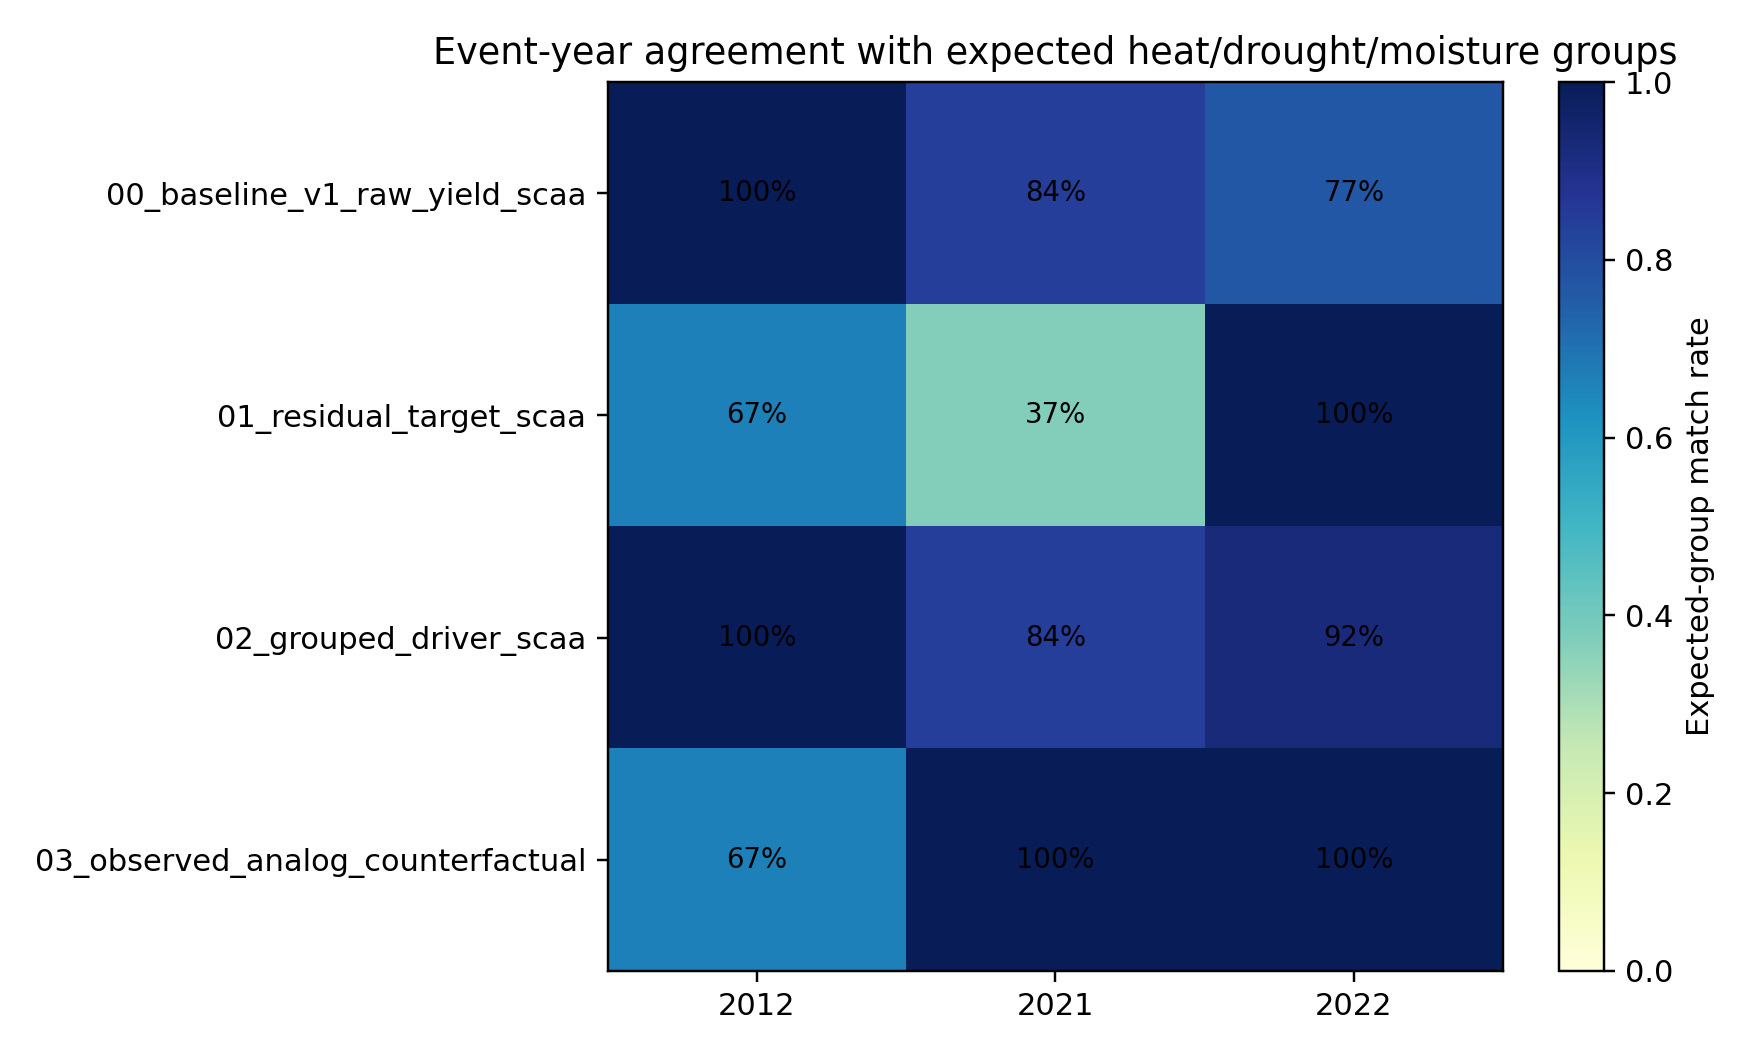
\includegraphics[width=0.9\linewidth]{fig08_event_validation.png}
  \caption{Event-year consistency with pre-specified heat, drought, and moisture stress groups.}
  \label{fig:event_consistency_supp}
\end{figure}

\section{Early-Warning Extension}
\begin{table}[!htbp]
\centering
\caption{Numeric early-warning performance corresponding to Figure 9.}
\label{tab:early_warning_metrics}
\resizebox{\linewidth}{!}{%
\begin{tabular}{lllllll}
\toprule
stage & roc\_auc & average\_precision & brier\_score & top\_10\_precision & top\_20\_precision & threshold\_from\_calibration \\
\midrule
Early-season & 0.473 & 0.225 & 0.216 & 0.208 & 0.229 & 0.14 \\
Early + mid-season & 0.597 & 0.301 & 0.185 & 0.333 & 0.333 & 0.16 \\
\bottomrule
\end{tabular}%
}
\end{table}


\begin{figure}[H]
  \centering
  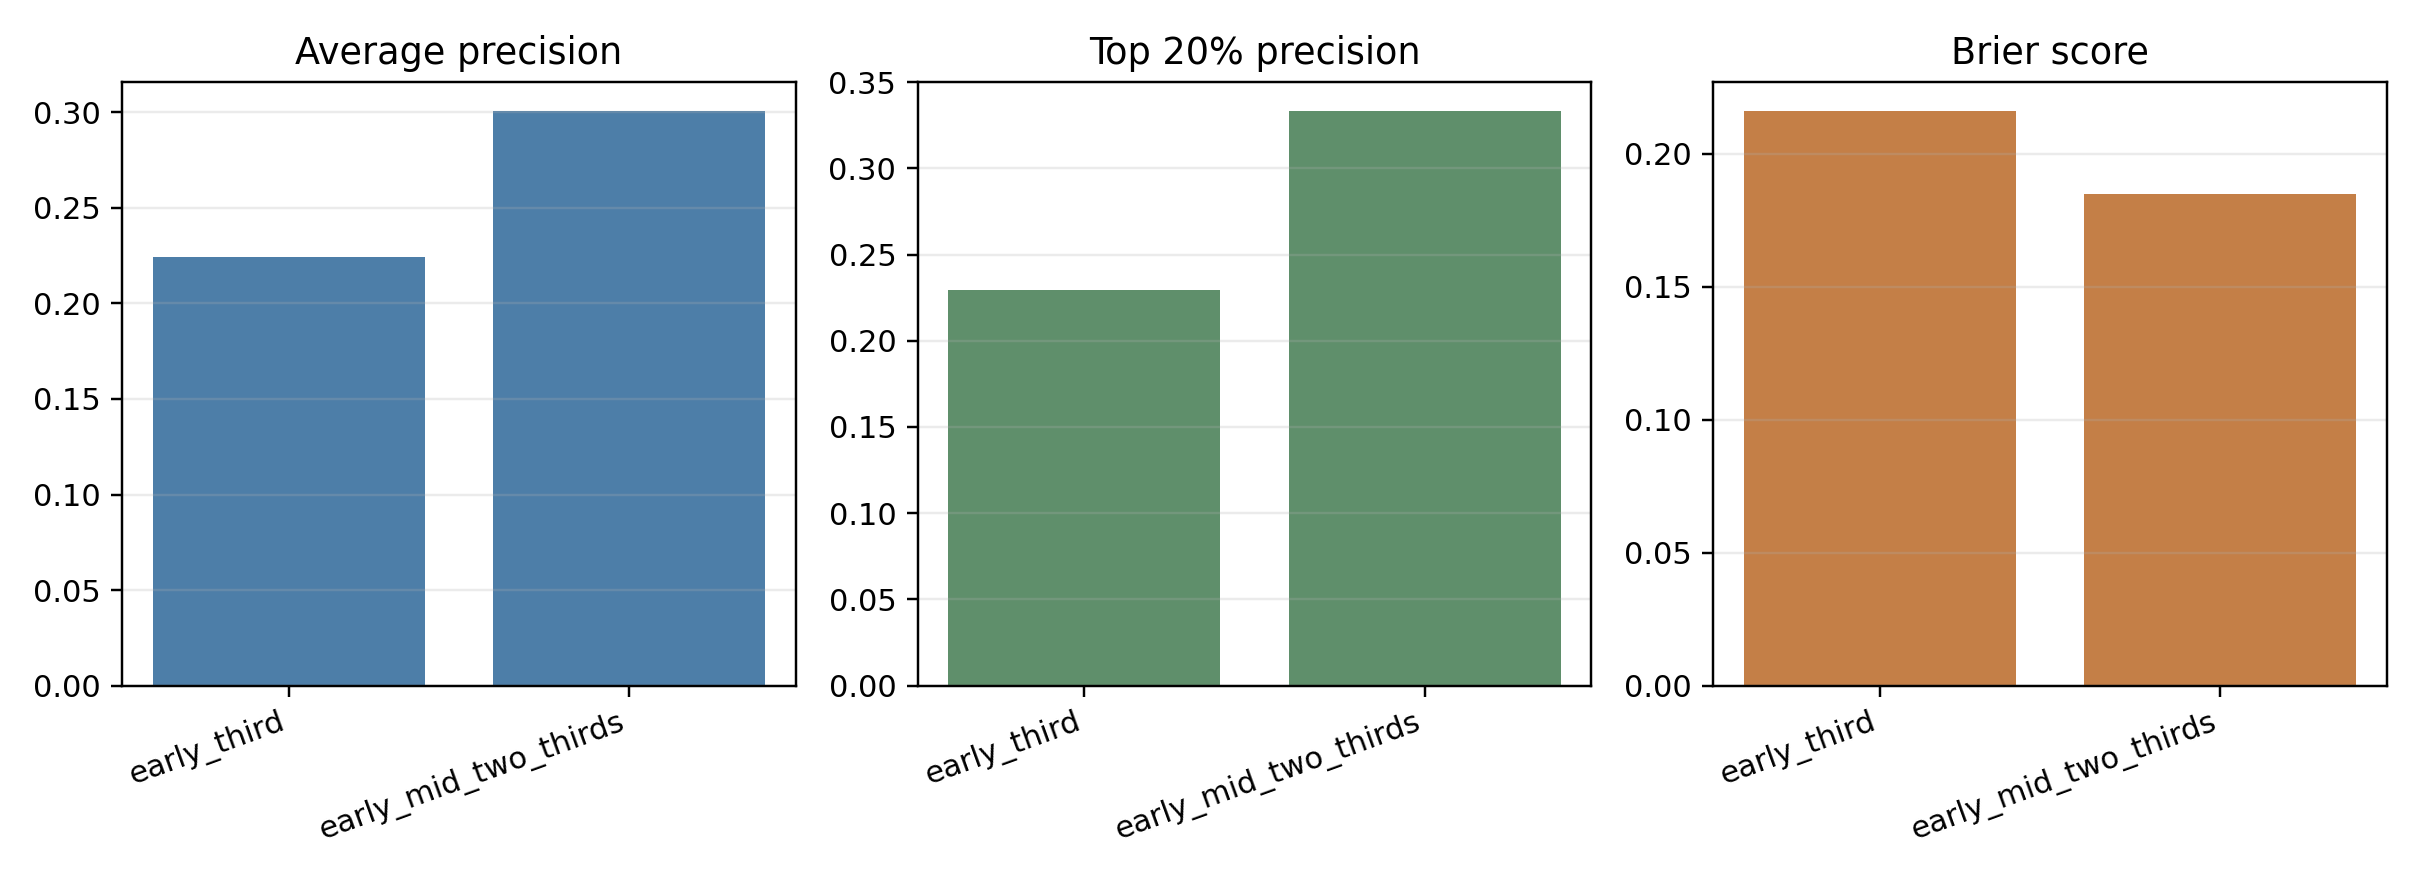
\includegraphics[width=\linewidth]{fig09_early_warning.png}
  \caption{Early-warning extension comparing early-season and early-plus-mid-season anomaly risk models.}
  \label{fig:warning_supp}
\end{figure}

\section{Reference Mapping}
\begin{table}[H]
\centering
\caption{Reference mapping to manuscript sections.}
\label{tab:reference_mapping}
\small
\renewcommand{\arraystretch}{1.15}
\begin{tabularx}{\linewidth}{@{}>{\raggedright\arraybackslash}p{0.18\linewidth}>{\raggedright\arraybackslash}p{0.34\linewidth}X@{}}
\toprule
paper section & use & bib keys \\
\midrule
Introduction & Extreme weather and crop-yield losses & Lesk2016; Zampieri2017; Vogel2019; Ray2015 \\
Related work & Machine-learning crop-yield prediction & Paudel2021; Meroni2021; Khaki2019; LengHall2020 \\
Related work & Yield anomalies and detrending & Lu2017; Ray2015; Meng2024; Sjulgard2023 \\
Related work & Interpretable ML for yield models & LundbergLee2017; Ribeiro2016; Mohan2025 \\
Method & Sparse and feasible counterfactual explanation & Wachter2018; Mothilal2020; Ustun2019; Poyiadzi2020; Verma2024 \\
Method and limitations & Event-attribution language and pitfalls & Hannart2016; Otto2017; Oldenborgh2021; OrtizBobea2021 \\
Data & Weather and yield data sources & NASAPOWER2025; USDANASSQuickStats \\
Extension & Early warning and conformal uncertainty & Anderson2024; Meroni2021; Singh2024; Farag2025 \\
\bottomrule
\end{tabularx}
\end{table}


\end{document}
